% Training-image grid — 6 representative PlantCLEF~2024 single-plant
% images, 2 rows x 3 columns. The image filenames are content hashes
% from the PC24 distribution; no species captions are shown here
% (species are described in the host caption).
%
% Required host preamble:
%   \usepackage{graphicx}
%   \usepackage{tikz}

\begin{tikzpicture}[
  every node/.style={inner sep=0pt, outer sep=0pt},
]

\def\cellw{50mm}
\def\cellh{50mm}
\def\colsep{2mm}
\def\rowsep{3mm}

% ── Row 1 ──────────────────────────────────────────────────────────────
\node                                       (t1) at (0, 0) {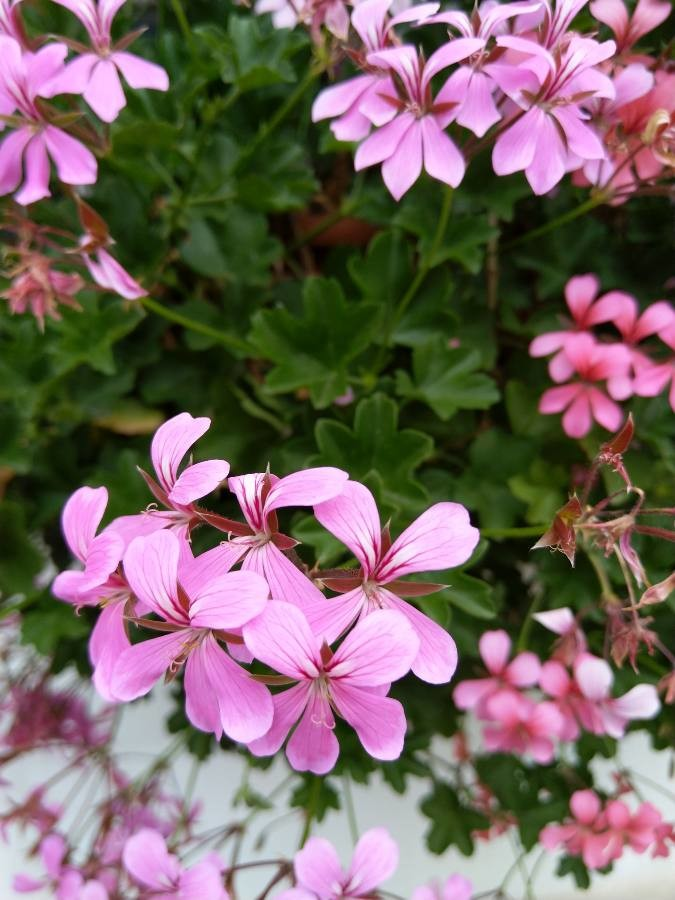
\includegraphics[width=\cellw, height=\cellh, keepaspectratio]{images/train/0b4007a0ea47ce9a04625baca25ce8b31eaafb44.jpg}};
\node[right=\colsep of t1.east, anchor=west](t2)            {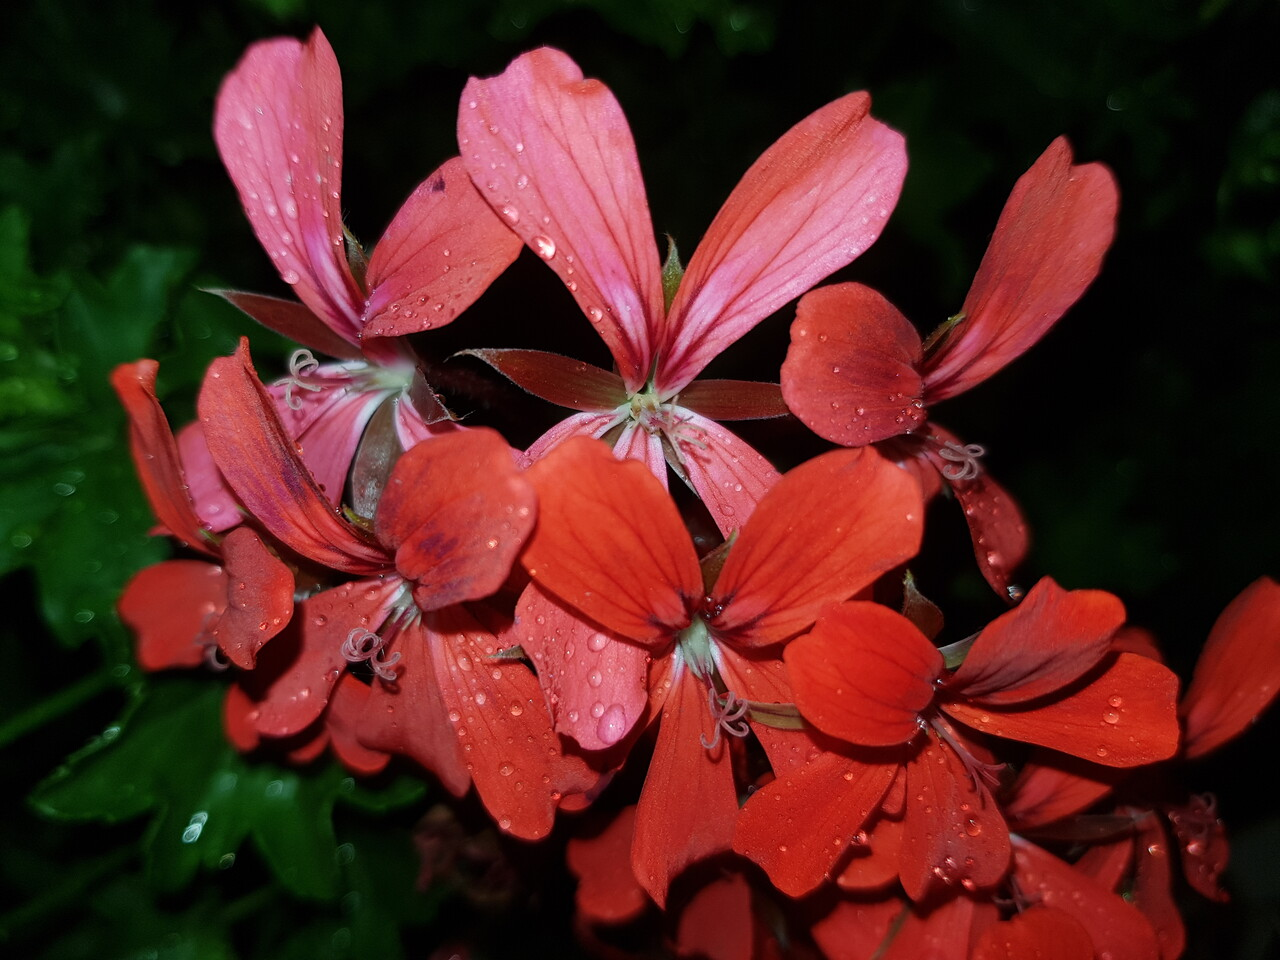
\includegraphics[width=\cellw, height=\cellh, keepaspectratio]{images/train/0b5296be0cd6e68cf46f7331edbc54ae600a0f1d.jpg}};
\node[right=\colsep of t2.east, anchor=west](t3)            {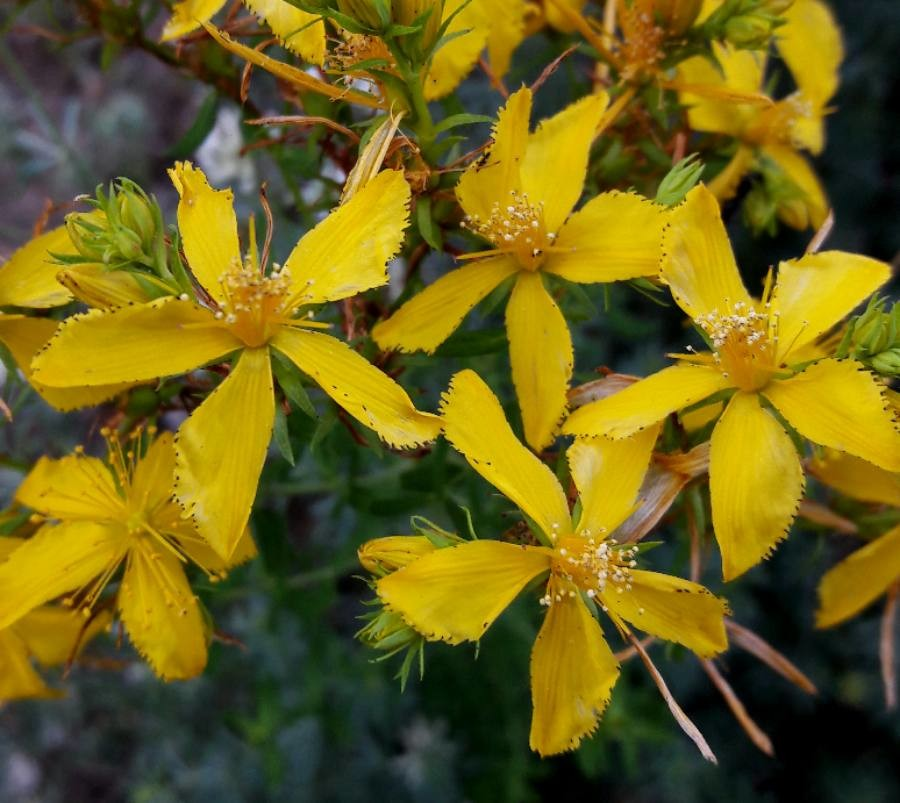
\includegraphics[width=\cellw, height=\cellh, keepaspectratio]{images/train/0c5ab5fd302458218691c7833a97688793a7466f.jpg}};

% ── Row 2 ──────────────────────────────────────────────────────────────
\node[below=\rowsep of t1.south, anchor=north]              (t4) {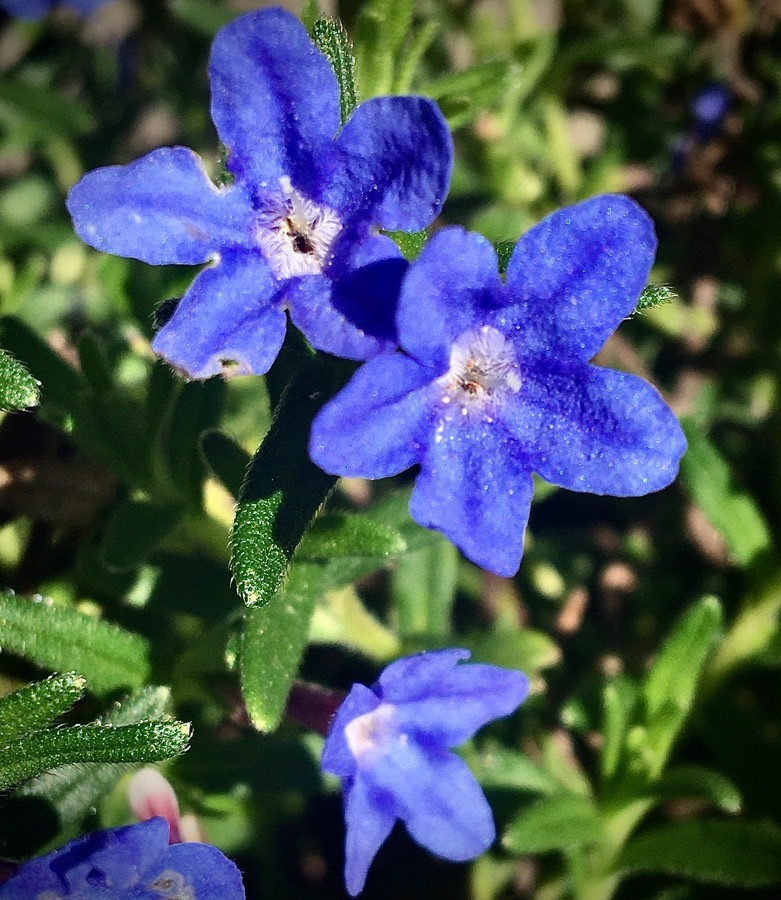
\includegraphics[width=\cellw, height=\cellh, keepaspectratio]{images/train/3f2b6248fa328d486b33b4f77f65d6b18b74c5c6.jpg}};
\node[right=\colsep of t4.east, anchor=west]                (t5) {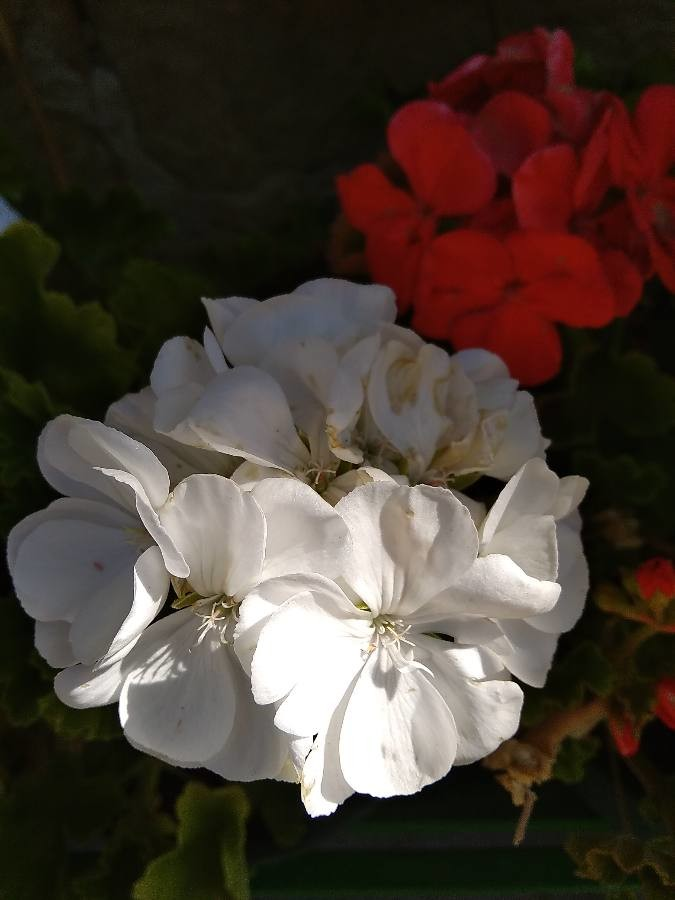
\includegraphics[width=\cellw, height=\cellh, keepaspectratio]{images/train/9cf6b7997a95b2bab8d840e70397b98dc8321106.jpg}};
\node[right=\colsep of t5.east, anchor=west]                (t6) {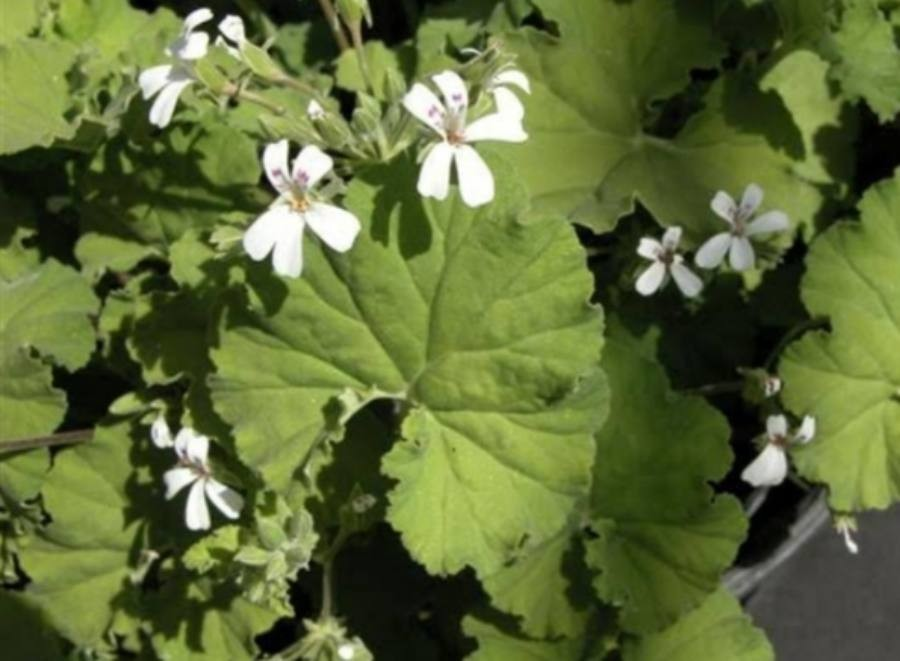
\includegraphics[width=\cellw, height=\cellh, keepaspectratio]{images/train/fe3131163544feb319ec6754b79ca33007177e95.jpg}};

\end{tikzpicture}
